\chapter{État de l'art sur la similarité moléculaire}
\label{chap2}

La similarité moléculaire joue un rôle important dans de nombreux aspects de la chémo-informatique tels que la recherche de similarité, la classification de bases de données moléculaires, la découverte de médicaments et l'analyse de la diversité moléculaire. La similarité englobe les positions atomiques, les conformations, la forme et la disposition spatiale des propriétés moléculaires\cite{dean2012molecular}. 

Cependant, la similarité entre deux molécules doit être optimisée par rapport aux applications examinées. C'est un domaine large et en constante évolution. Il existe de multiples mesures de similarité décomposés entre autre en ceux qui sont basés sur le graphe moléculaire, ceux qui basés de la conformation et ceux qui demandent un calcul de la fonction d'onde moléculaire. On distingue: 

\begin{itemize}
\item Les \textbf{mesures unidimensionnelles}\cite{dixon2001one} sont basées sur les propriétés physico-chimiques des molécules telles que le volume, la polarisation et le poids. Puisqu'elles ne prennent pas en considération les informations géométriques de la molécules, ces mesures sont généralement utilisés pour le clustering des bases de données\cite{downs1994similarity}.

\item Les \textbf{mesures $2D$} sont basées sur le graphe moléculaire. La mesure la plus répandue pour comparer les structures chimiques représentées en utilisant les empreintes est le coefficient de Tanimoto \cite{bajusz2015tanimoto}. La recherche de sous-structure via la sous-structure commune maximum (en anglais, Maximum Common Subgraph MCS\cite{rascal} se classe aussi dans cette catégorie.

\item Les  \textbf{mesures 3D} tel que l'empreinte $3D$ utilisent l'alignement des molécules dans l'espace. Contrairement aux méthodes $1D$ et $2D$, elles tiennent compte de la taille et de la forme des structures moléculaires (propriétés conformationnelles) \cite{shin2015three}.
Cependant, elles restent moins utilisées car beaucoup plus complexes\cite{bero2017similarity, barbosa}.

%empreintes 3D : pharmacophore fingerprints
\end{itemize}
La similarité que nous recherchons durant la thèse se situe sur la partie structurelle notamment les mesures $2D$ sur les graphes moléculaires. Dans la section \ref{tanimoto}, nous présenterons le quelques mesures de similarité basés sur le calcul d'empreintes dans le graphe moléculaire, plus précisement le coefficient de Tanimoto. Ensuite dans la Section \ref{mces}, nous exposerons la mesure de similarité basée sur le problème Maximum Common Edge Subgraph. 
%suites binaires = empreintes

%Dans ce chapitre, nous allons présenter quelques mesures de similarité

Ce chapitre contient également dans la Section \ref{theoriegraphe}, les définitions préliminaires sur les notions de cycles, bases de cycles, union de bases de cycles dans les graphes. Ces notions de la théorie de graphes seront utilisés dans les chapitres suivants. 


\section{Les mesures de similarité basés sur les empreintes}
\label{tanimoto}

Les empreintes ou suites binaires sont calculées à partir de la présence ou de l'absence de caractéristiques moléculaires. Elles sont généralement comparées en utilisant un coefficient de similarité en tant que mesure de la similarité entre les structures. %Cette méthode est particulièrement efficace dans le cas où les motifs sont faciles à calculer.

Pour calculer la similarité il faut dans un premier temps associer à chaque molécule, une empreinte. Dans un second temps choisir le coefficient adapté pour obtenir une mesure. 

\subsection{Le calcul des empreintes}

Les principales types d'empreintes sont les empreintes basées sur les notions de sous-structures, les empreintes topologiques ou basées sur le chemin, et les empreintes circulaires.


\begin{itemize}
\item Les empreintes basées sur des motifs (sous- structures) définissent les bits l'empreinte en fonction de la présence dans le composé de certaines sous-structures ou caractéristiques d'une liste donnée de motifs. Ces empreintes sont intéressantes lorsqu'elles sont utilisées avec des molécules susceptibles d'être recouvertes par la liste de motifs choisie. Elles le sont moins lorsque les molécules contiennent d'autres motifs, car leurs présence ne seraient pas représentés. Leur nombre de bits de l'empreinte est déterminé par le nombre de motifs, et chaque bit renseigne sur la présence ou à l'absence d'une caractéristique donnée dans la molécule. %Les motifs sont généralement 

\item Les empreintes topologiques analysent tous les fragments de la molécule en parcourant un chemin linéaire jusqu’à un certain nombre de liaisons, puis en hachant chacun de ces chemins pour créer l’empreinte. Ainsi toute molécule peut produire une empreinte digitale cohérente et sa longueur peut être ajustée. Ce type d'empreintes est utilisé pour la recherche de sous-structures. L’empreinte la plus connu sous le nom de Daylight \cite{} comporte jusqu'à 2048 bits et code toutes les motifs possibles à travers une molécule jusqu'à une longueur donnée.

\item Les empreintes circulaires ressemblent aux empreintes topologiques à la différence qu'au lieu de rechercher des chemins dans le graphe moléculaire, ils stockent l'environnement de chaque atome jusqu'à un rayon fixé. On distingue parmis les empreintes cirulaires : Extended-Connectivity Fingerprint (ECFP diamètre $4$ et $6$) basé sur l'algorithme de Morgan, Functional-Class Fingerprints (FCFP $4$ et $6$) et Molprint2D.

\end{itemize}
\subsection{Coefficients de similarité}
Les mesures de similarité suivantes supposent que deux empreintes avec de nombreux bits en commun sont similaires. Ce sont des mesures brutes mais étonnamment efficaces pour une large gamme d'applications.

En effet, l'information de présence ou d'absence d'un motif est moins exhaustive que le nombre d'occurrences de celui-ci, ce qui, à son tour, ne donne aucune information sur la façon dont les motifs survenus sont répartis dans la molécule. %Les descripteurs 2D ou topologiques capturent les informations relatives à la connectivité moléculaire, caractérisant formellement le graphe représentant le schéma de connexion interatomique dans la molécule. 

Le tableau \ref{tableauempreintes} présente les différentes mesures et distances connues pour obtenir un coefficient de similarité. La plus utilisée est le coefficient de Tanimoto qui consiste à faire le ratio entre le nombre de bits communs à $1$ et le nombbre total de bits à $1$ dans les deux empreintes. Ce coefficient est compris dans $[0,1]$ quelque soit la taille des empreintes. 

\begin{center}

\begin{table}[!ht]

\label{tableauempreintes}
\centering
\caption{
{\bf Coefficients de similarité et distance basés sur les empreintes}}
\begin{tabular}{|c|c|c|}
%\caption{\textbf{Coefficients de similarité et distance basés sur les empreintes}.   }
\hline
\textbf{Mesure de similarité }& \textbf{Intervalle} & \textbf{Formule} \\
\hline
\textbf{Similarité de Cosine}& $[0,1]$ & $\frac{c}{\sqrt{a\times b}}$\\
\hline
\textbf{Coefficient de Tanimoto}& $[0,1]$ & $\frac{c}{\sqrt{a+ b - c}}$\\
\hline
\textbf{Coefficient de Dice }& $[0,1]$ & $\frac{2 \times c}{\sqrt{a+ b}}$\\
\hline
\textbf{Distance euclidienne}& $[0,N]$ & $\sqrt{a + b - 2 \times c}$\\
\hline
\textbf{Distance de Hamming}& $[0,N]$ & $a + b - 2 \times c$\\
\hline
\textbf{Coefficient de Forbes}& $[0,1]$ & $\frac{c \times m}{
a \times b }$\\
\hline
\textbf{Distance de Soergel }& $[0,1]$ & $\frac{a + b - 2 \times c}{\sqrt{a+ b - c}}$\\
\hline


\end{tabular}
\vspace*{0.4cm}

On considère deux empreintes moléculaires $A$ et $B$. On note $m$, le nombre total de bits dans $A$ et $B$; a, b et c représente respectivement le nombre de bits à $1$ dans $A$, le nombre de bits à $1$ dans $B$ et le nombre de bits à $1$ à la fois dans $A$ et $B$.

\end{table}
\end{center}

\textcolor{red}{exemple de calcul Tanimoto ?}


\section{Similarité basé sur le Maximum Common Edge Subgraph (MCES)}
\label{mces}
Dans cette section, nous allons présenter le calcul de similarité basé sur la recherche de sous-graphe commun ayant un nombre maximum d'arêtes. Toutefois nous nous limiterons à la définition de la mesure exacte et nous n'allons pas présenter les heuristiques[refs].

Soient deux graphes moléculaires $G_1=(V_1,E_1)$ et $G_2=(V_2,E_2)$. 

\begin{definition}
Un \textit{sous-graphe commun induit} $G_{1,2}$ de $G_1$ et $G_2$ est un graphe isomorphe à des sous-graphes induits de $G_1$ et $G_2$. Un graphe $G_{1,2}$ est un sous-graphe commun induit maximum (MCIS) s'il contient un nombre maximum de sommets dans $G_1$ et $G_2$. Un graphe $G_{1,2}$ est un sous-graphe commun ayant un nombre d'arêtes maximum (MCES) s'il contient un nombre maximum d'arêtes communs dans $G_1$ et $G_2$.
\end{definition}

Un MCIS et un MCES peuvent être des sous-graphes non connexes.
\begin{figure}[H]
\label{mcis-mces}

\caption{(a) Deux graphes $G_1$ et $G_2$, (b) en gras un MCIS et (c) en gras un MCES.}
\begin{center}
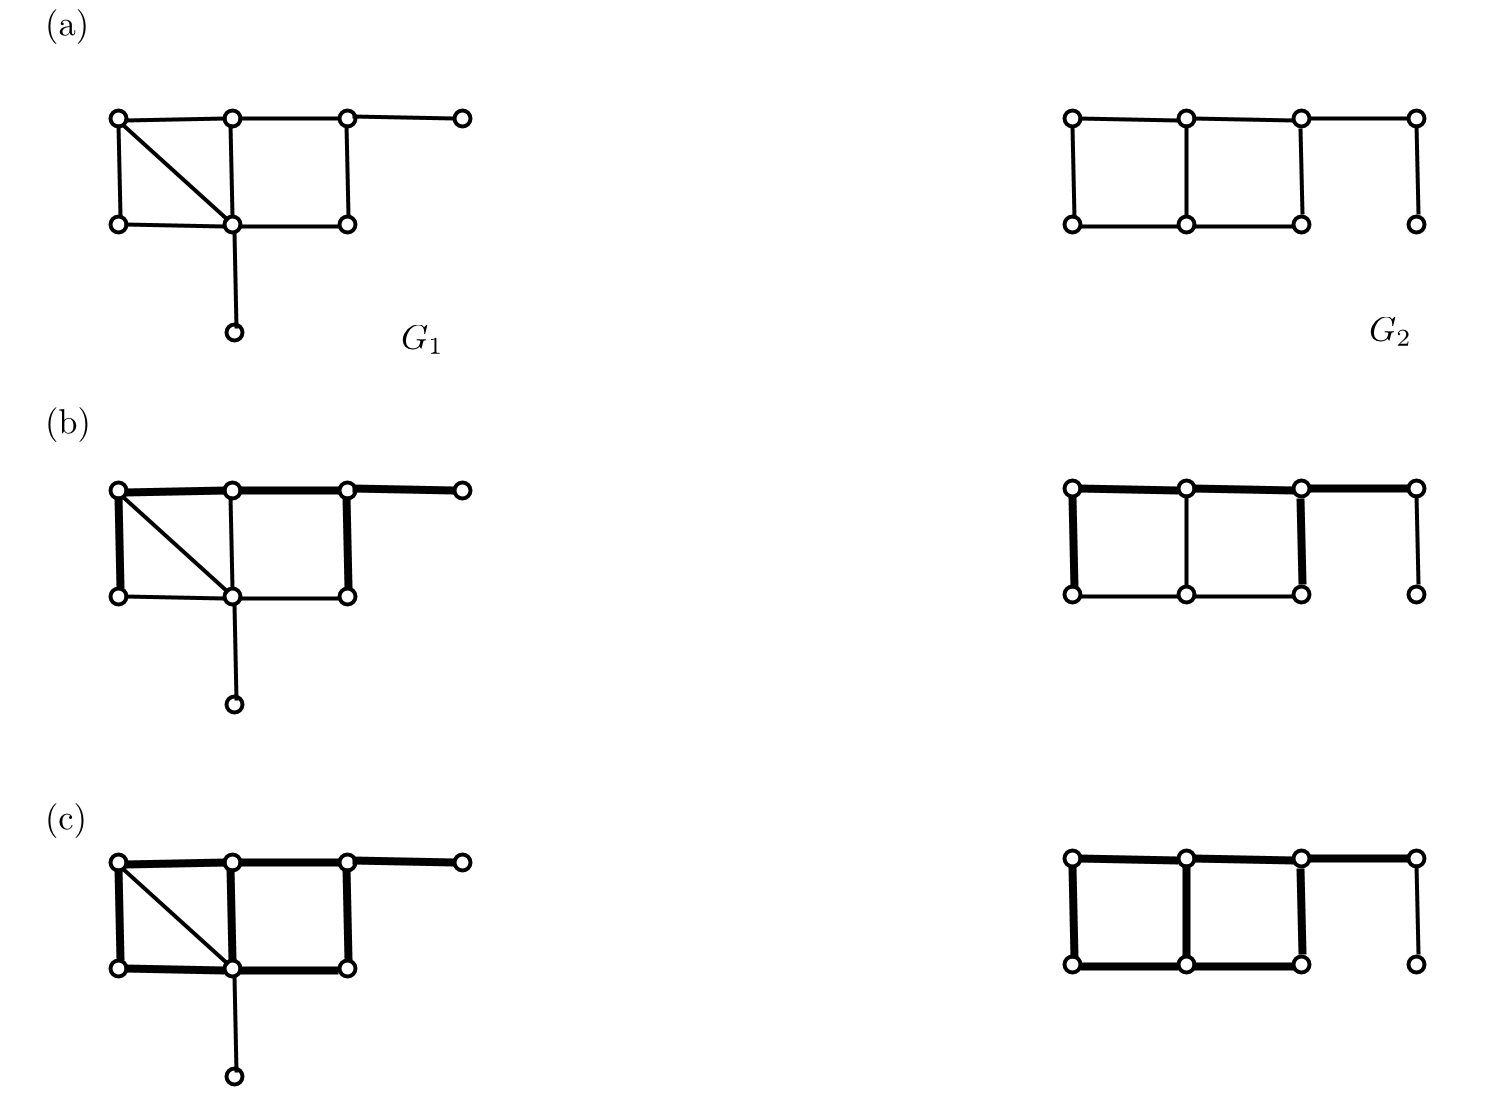
\includegraphics[scale=0.5]{mces_mcis.png}
\end{center}
\end{figure}

Pour le calcul de similarité trouver un sous-graphe commun ayant un nombre d'arêtes maximum  est pertinent \cite{rascal}. Dans la suite, on note $G_{1,2}=(V_{1,2},E_{1,2})$ un sous-graphe commun ayant un nombre maximum d'arêtes à la fois dans $G_1$ et $G_2$. La mesure de similarité $\mathrm{sim(G_{1},G_{2})}$ est :

\begin{eqnarray}
\mathrm{sim(G_{1},G_{2}) }= \frac{(|V _{12}| + |E _{12}| )^2 }{(|V _1| + |E_1| )\times (|V_2| + |E _2| )}
\label{eq:mces}
\end{eqnarray}

La recherche d'un sous-graphe commun ayant un nombre maximum d'arêtes se fait en trois étapes : le calcul du graphe produit, la recherche d'une clique maximum et l'extraction d'un sous-graphe commun à arêtes maximum entre $G_1$ et $G_2$.

\subsection{Le calcul du graphe moléculaire produit }

La première étape consiste à calculer le graphe moléculaire produit des linegraphes $G_1$ et de $G_2$ noté $L(G_1)\diamond (G_2)$. Le linegraphe $L(G_1)$ d'un graphe $G_1$ est un graphe dans lequel les arêtes de $G_1$ sont des sommets et deux sommets de $L(G_1)$ sont adjacents si et seulement si les arêtes correspondantes dans $G_1$ sont adjacentes.
Ce graphe moléculaire produit est telle que : $V(G_1\diamond G_2) = V(L(G_1)) \times V(L(G_2))$.

Soient deux sommets $(u_i,v_i), (u_j,v_j)  \in V(L(G_1)\diamond L(G_2))$. L'arête $[(u_i,v_i), (u_j,v_j)] \in E(L(G_1)\diamond L(G_2))$ si et seulement si :

\begin{itemize}
\item $(u_i,u_j) \in E(L(G_1))$, $(v_i,v_j) \in E(L(G_2))$ et $w(u_i,u_j)= w(v_i,v_j)$ \textbf{OU}
\item $(u_i,u_j) \notin E(L(G_1))$, $(v_i,v_j) \notin E(L(G_2))$.
\end{itemize}
La fonction $w(u_i,u_j)= w(v_i,v_j)$ vérifie la compatibilité entre les atomes et les liaisons. Elle associe les atomes et les liaisons du même type.

\begin{exemple}
On considère deux graphes moléculaires $G_1$ et $G_2$ de la Figure \ref{produit}(a). Les Figures  \ref{produit}(b) et \ref{produit}(c) montrent respectivement le calcul du linegraph des graphes  et les sommets du graphe produit.

\begin{figure}[H]
\label{produit}
\begin{center}
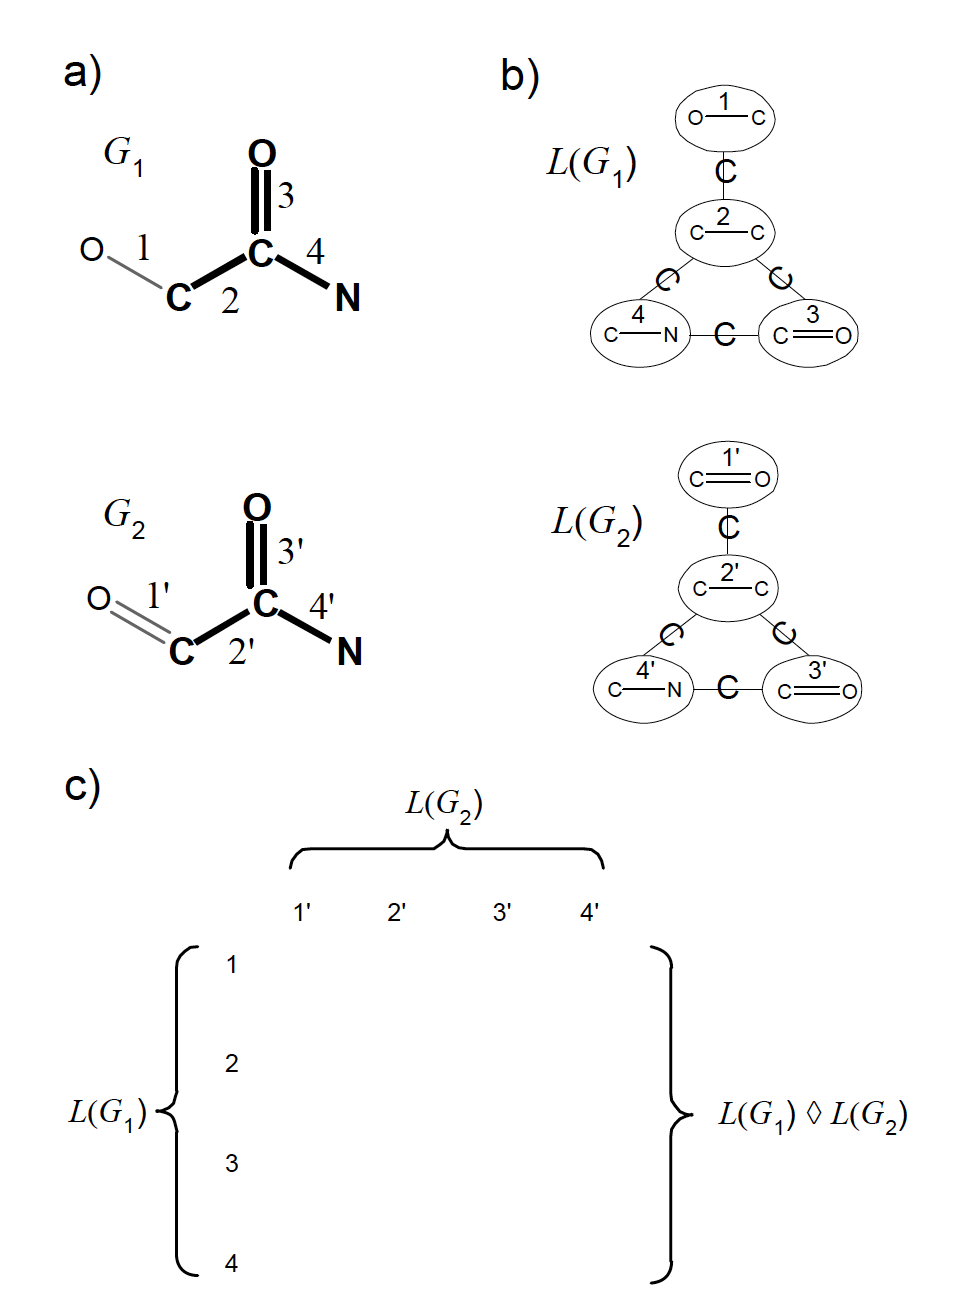
\includegraphics[scale=0.65]{produit.png}
\caption{Construction d'un graphe moléculaire produit}
\end{center}
\end{figure}
\end{exemple}

\subsection{La recherche d'une clique maximum et l'extraction d'un sous-graphe commun à arêtes maximum}

En utilisant le graphe produit des linegraphes de $G_1$ et $G_2$, on recherche une clique maximum à partir de laquelle on extrait un sous-graphe commun à arêtes maximum.

\begin{exemple}
En reprenant le graphe moléculaire produit de l'exemple précédent, on cherche une clique maximum.
\begin{table}[!ht]
\begin{flushleft}


\begin{tabular}{|p{1.0cm}|*{17}{@{\hskip.01mm}c@{\hskip.01mm}|}}
\hline
&$(1,1')$&$(1,2')$&$(1,3')$&$(1,4')$&$(2,1')$&$(2,2')$&$(2,3')$&$(2,4')$&$(3,1')$&$(3,2')$&$(3,3')$&$(3,4')$&$(4,1')$&$(4,2')$&$(4,3')$&$(4,4')$\\\hline
$(1,1')$&1&0&0&0&0&0&0&0&0&0&1&0&0&0&0&1\\ \hline
$(1,2')$&0&1&0&0&0&0&0&0&0&0&0&0&0&0&0&0\\ \hline
$(1,3')$&0&0&1&0&0&0&0&0&0&0&0&0&0&0&0&0\\ \hline
$(1,4')$&0&0&0&1&0&0&0&0&0&0&0&0&0&0&0&0\\ \hline
$(2,1')$&0&0&0&0&1&0&0&0&0&0&0&0&0&0&0&0\\ \hline
$(2,2')$&0&0&0&0&0&1&0&0&0&0&1&0&0&0&0&1\\ \hline
$(2,3')$&0&0&0&0&0&0&1&0&0&1&0&0&0&0&0&0\\ \hline
$(2,4')$&0&0&0&0&0&0&0&1&0&0&0&0&0&0&0&0\\ \hline
$(3,1')$&0&0&0&0&0&0&0&0&1&0&0&0&0&0&0&0\\ \hline
$(3,2')$&0&0&0&0&0&0&1&0&0&1&0&0&0&0&0&0\\ \hline
$(3,3')$&1&0&0&0&0&1&0&0&0&0&1&0&0&0&0&1\\ \hline
$(3,4')$&0&0&0&0&0&0&0&0&0&0&0&1&0&0&1&0\\ \hline
$(4,1')$&0&0&0&1&0&0&0&0&0&0&0&0&1&0&0&0\\ \hline
$(4,2')$&0&0&0&0&0&0&0&1&0&0&0&0&0&1&0&0\\ \hline
$(4,3')$&0&0&0&0&0&0&0&0&0&0&0&1&0&0&1&0\\ \hline
$(4,4')$&1&0&0&0&0&1&0&0&0&0&1&0&0&0&0&1\\ \hline

\end{tabular}
\end{flushleft}
\end{table}

On trouve une clique maximum de taille $3$. La taille de la clique est égale au cardinal de $E(G_{12})$. On fait ensuite une projection des arêtes de la clique dans $G_1$( ou $G_2$) pour obtenir un sous-graphe commun ayant un nombre maximum d'arêtes à la fois dans $G_1$ et $G_2$. Dans cet exemple, on a :
\begin{itemize}
\item $|V(G_1)| = 5$ et $|E(G_1)| = 4$
\item $|V(G_2)| = 5$ et $|E(G_2)| = 4$
\item $|V(G_{12})| = 4$ et $|E(G_{12})| = 3$


\end{itemize}
\begin{center}


 $\mathrm{sim(G_{1},G_{2}) }= \frac{(4 + 3 )^2 }{(5 + 4 )\times(5 + 4 )} = 0,6$
 \end{center}
\end{exemple}
La recherche de clique maximum est un problème NP-Complet. Il existe des heuristiques tels que les algorithmes de branch and bound \cite{rascal}.

\section{Quelques préliminaires de la théorie de graphes}
\label{theoriegraphe}
Dans cette section, nous allons définir quelques notions de la théorie de graphes \textcolor{red}{ (ref claude berges graph theory and application)} que nous utiliserons dans les chapitres suivants. Les informations sur les cycles constituent une partie importante de la topologie structurelle utilisée pour identifier et caractériser les structures moléculaires. Il est donc d’une importance cruciale d’obtenir ces informations pour diverses tâches en chimie computationnelle.

On considère un graphe simple et non orienté $G = (V, E)$ avec $n$ et $m$ respectivement le nombre de sommets et le nombre d 'arêtes de $G$. On note $V = \{v_1, v_2, ..., v_n\}$ avec $v_i$ le sommet d'indice $i$ et l'ensemble $E= \{e_1, e_2, ..., e_m\}$ tel que $e_j = [v_i, v_i']$.

\subsection{Chaînes et cycles}

\begin{definition}
Une chaîne est une suite fini d'arêtes consécutives $e_1, e_2, ...,e_k$ de $G$. La longueur d'une chaîne est le nombre d'arêtes qui la composent.
\end{definition}

Une chaîne est élémentaire si et seulement si elle passe au maximum une fois par chaque sommet. Une chaîne simple est une chaîne ne passant pas deux fois par une même arête.

\begin{definition}
Un cycle est une chaîne simple dont les extrémités sont identiques. Un cycle élémentaire ne contient pas d'autres cycles.
\end{definition}

Nous allons représenter un cycle élémentaire $c$ par un vecteur $v_c = (e_1^{c}, e_2^{c}, ...., e_m^{c})$ de taille $m$ avec $e_i^c = 1$ si et seulement si $e_i^c \in c$ et $e_i^c = 0$ sinon. La longueur d'un cycle notée $|c|$ vaut $\sum_{i = 1}^{m}e_i^c$.

\begin{exemple}
\label{exemplecycles}
Soit le graphe $G$ de la Figure \ref{chainescycles} avec $V = \{v_1, v_2, v_3, ...,v_9, v_{10}\}$ et $E = \{e_1, e_2, ...,e_{10}, e_{11}\}$. La chaîne $(e_1, e_2, e_3, e_4)$ est une chaîne élémentaire de $G$. Les cycles $c_1 =(e_1, e_2, e_{11}, e_8, e_9, e_{10})$ et $c_2 =(e_3, e_4, e_5, e_6, e_7,e_{11})$ sont des cycles élémentaires dont les vecteurs sont respectivement : 

\begin{center}
$v_{c_1} = (1, 1, 0, 0, 0, 0, 0, 1, 1, 1, 1)$\\
$v_{c_2} = (0, 0, 1, 1, 1, 1, 1, 0, 0, 0, 1)$

\end{center}
\begin{figure}[H]
\label{chainescycles}
\begin{center}
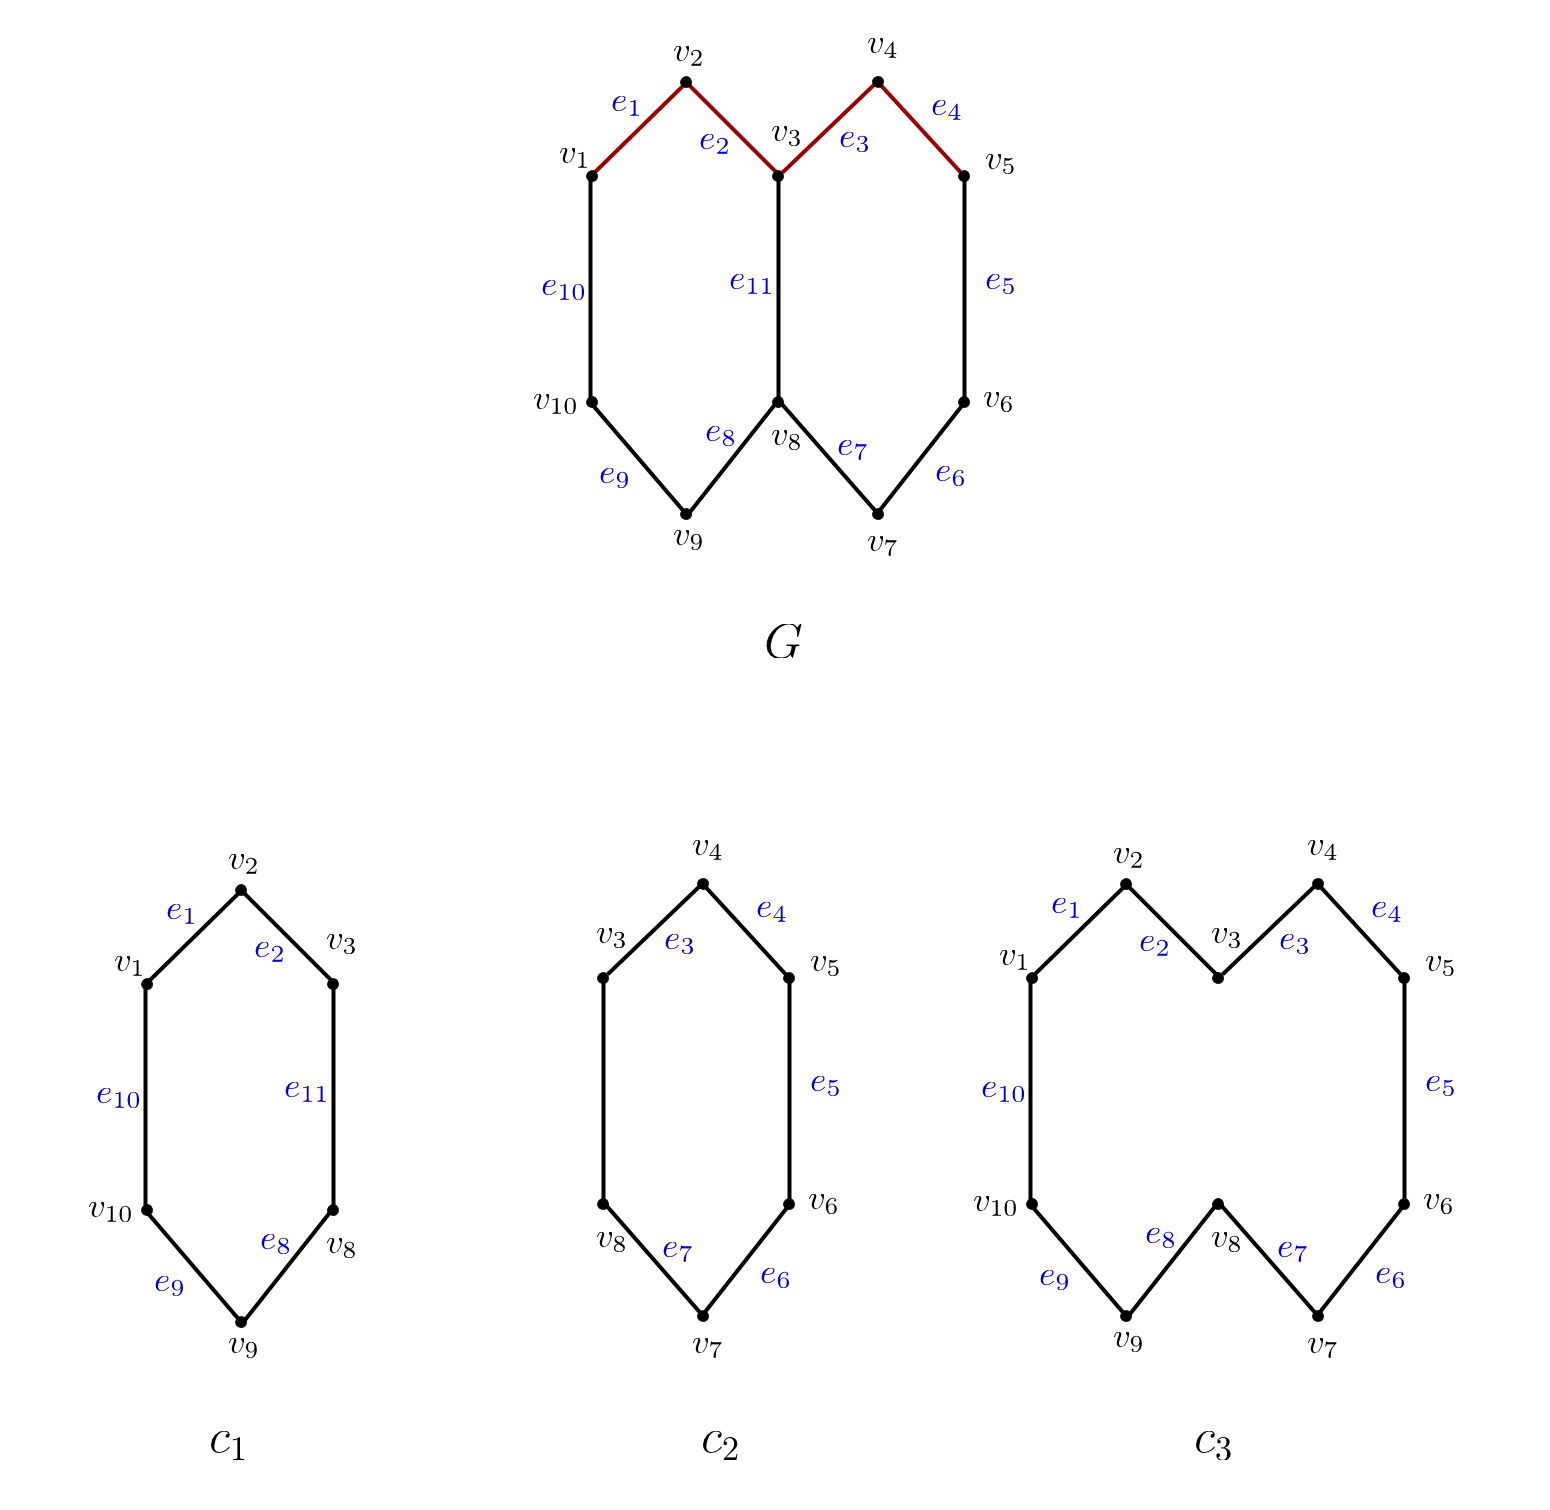
\includegraphics[scale=0.42]{chainescycles.png}
\end{center}
\caption{Chaînes et cycles élémentaires dans un graphe }
\end{figure}
\end{exemple}

On considère deux cycles élémentaires $c_1$ et $c_2$ dans un graphe $G$ telle que : $v_{c_1} = (e_1^{c_1}, e_2^{c_1}, ...., e_m^{c_1})$ et $v_{c_2} = (e_1^{c_2}, e_2^{c_2}, ...., e_m^{c_2})$.

\begin{definition}
L'union disjointe des cycles $c_1$ et $c_2$ notée $c_{12}$ est la différence symétrique des arêtes du graphe appartenant à $c_1$ et $c_2$. On note $c_{12} = c_1 \oplus c_2$ et le vecteur associé est $v_{c_{12}} = (e_1^{c_1} \oplus e_1^{c_2}, e_2^{c_1} \oplus e_2^{c_2}, ...., e_m^{c_1} \oplus e_m^{c_2})$.
\end{definition}

L'opérateur $\oplus$ représente le XOR binaire sur les $e_i^c$. L'union de deux cycles disjoints donne un vecteur composé de deux cycles disjoints. Dans l'Exemple \ref{exemplecycles}, le cycle $c_3$ est l'union disjointe des cycles $c_1$ et $c_2$.

%Le nombre cyclomatique
Lorsque dans un graphe, deux sommets d'un cycle sont reliés par une arête qui n'appartient pas au cycle, cette arête est appelée \textit{corde} du cycle. Un cycle de G dit induit lorsqu'il n'a pas de cordes.

\begin{definition}
Un cycle est dit \textbf{pertinent} s'il ne peut pas être obtenu par combinaison de cycles de longueur strictement plus petite.
\end{definition}

\subsection{Connexité et isthme}

\begin{definition}
Un graphe $G$ est \textbf{connexe} si toute paire de sommets $u,v \in V$ peut être reliée par une chaîne dans $G$.
\end{definition}
Un sous-graphe connexe maximal de $G$ est appelé composante connexe de $G$. Un graphe qui n'est connexe possède au moins $2$ composantes connexes.

%Un graphe connexe qui reste connexe après suppression de n’importe quel sous-ensemble de $k − 1$ sommets est dit $k-$connexe. 
Soit un graphe connexe $G$ et un ensemble d'arêtes $E'$ de $G$. Si le graphe $G -  E'$ n'est pas connexe, on dit que $E'$ est un séparateur de $G$. Si dans $G - E'$, deux sommets $u$ et $v$ sont dans deux composantes connexes différentes, on dit que $E'$ sépare $u$ de $v$ ou $E'$ est un $(u, v)-$séparateur.

\begin{definition}
 Pour $k \geq 1$, on dit que $G$ est $k-$connexe s'il a au moins $k+1$ sommets et aucun ensemble de $k -1$ sommets ne le sépare. Un graphe est k-arête-connexe, s'il a au moins deux sommets et aucun ensemble de $k - 1$ arêtes ne le sépare. 
\end{definition}

La valeur maximale $k$ pour laquelle une graphe G est $k - 1 $connexe est appelée connexité de $G$ et notée $\kappa(G)$. En particulier, lorsque $k = 2$ on parle de graphe $2-$connexe ou bi-connexe.
De même, la valeur maximale $k$ pour laquelle une graphe $G$ est $k-$arête-connexe est appelée arête-connexité de G et notée $\kappa′(G)$.

\begin{definition}
Une arête d'un graphe est un \textbf{isthme} si sa suppression augmente le nombre de composantes connexes du graphe. 
\end{definition}
Si le graphe est connexe, une arête est un isthme si et seulement si elle n'appartient à aucun cycle.

\subsection{Base de cycles}

Dans un graphe, on appele générateur de cycles $\zeta$, un ensemble fini de cycles tel que tout cycle de $G$ peut être obtenu par combinaison des cycles de $\zeta$.

\begin{definition}
On appelle une base de cycles $\mathcal{B}$, un ensemble de cycles linéairement indépendants et générateur.

\end{definition}

Soit $G$ un graphe de $n$ sommets, $m$ arêtes et $p$ composantes connexes,
la dimension d’une base de cycles est le nombre cyclomatique de $G: \nu(G)=m-n+p$. La longueur d'une base de cycles $\zeta$ est la somme des longueurs des cycles de la base. Il existe $2$ principales types de bases de cycles : les base de cycles fondamentales et les bases de cycles de longueurs minimum.

\subsubsection{Base de cycles fondamentale}

Lorsque le graphe $G$ est connexe, il est possible d'obtenir des bases de cycles en utilisant les arbres couvrants. Ces bases de cycles sont appelées \textbf{bases de cycles fondamentales} \cite{kir}.

Soit $T$ un abre couvrant arbitraire de $G$. Pour obtenir une base de cycles fondamentale, on rajoute à chaque fois à $T$, une arête de $G$ qui n'appartient pas à $T$. A chaque ajout, on cree un cycle qui appartient à la base de cycle fondamentale. On repète le procédé $m-n+1$ fois.

Cependant, trouver un abre couvrant tel que la base de cycles fondamentale soit minimum est un problème NP-Complet.

\subsubsection{Base de cycles de longueur minimum}

Une base de cycles de longueur minimum ou Mimimum Cycle Basis (MCB) est une base de cycles ayant une longueur minimale. Il existe plusieurs algorithmes pour trouver de telles bases. En chimie, les algorithmes developpés et applicables sur les structures moléculaires et graphes simples sont connus sous le nom de Smallest Set of Smallest Rings (SSSR)\cite{LeeJoon,Zamora,Qian}. En informatique, les algorithmes MCB d'une grande robustesse, sont concus pour des graphes en général \cite{horton,golynski2002polynomial,berger2004minimum,kavitha2004faster}.

Dans un graphe, il peut y avoir plusieurs bases de cycles de poids minimum. Lorsqu'il existe une unique base de cycles minimum $\mathcal{B}$ dans un graphe, cette base est aussi l'ensemble de cycles pertinents du graphe.

%\subsubsection{Ensembles de cycles pertinents}
\subsubsection{Union des bases de cycles de longueur minimum}


Également appelé ensemble de cycles pertinents, l'union des bases de cycles de longueur minimum est défini comme le plus petit ensemble canonique de cycles qui décrit la structure cyclique d'un graphe\cite{vismara}. Sa construction passe par l'obtention d'une représentation compacte servant de prototype pour les énumérer.